\documentclass[aspectratio=169]{beamer}
\usetheme[faculty=phil]{fibeamer}
\usepackage{polyglossia}
\setmainlanguage{english} %% main locale instead of `english`, you
%% can typeset the presentation in either Czech or Slovak,
%% respectively.
\setotherlanguages{russian} %% The additional keys allow
%%
%%   \begin{otherlanguage}{czech}   ... \end{otherlanguage}
%%   \begin{otherlanguage}{slovak}  ... \end{otherlanguage}
%%
%% These macros specify information about the presentation
\title[AGLA2]{Analytical Geometry and Linear Algebra II, Lab 7} %% that will be typeset on the
\subtitle{Complex numbers \\ Complex matrices \\ Hermitian and Unitary Matrices 
         } %% title page.
\author{Oleg Bulichev}
%% These additional packages are used within the document:
\usepackage{ragged2e}  % `\justifying` text
\usepackage{booktabs}  % Tables
\usepackage{tabularx}
\usepackage{tikz}      % Diagrams
\usetikzlibrary{calc, shapes, backgrounds}
\usepackage{amsmath, amssymb}
\usepackage{url}       % `\url`s
\usepackage{listings}  % Code listings
% \usepackage{subfigure}
\usepackage{floatrow}
\usepackage{subcaption}
\usepackage{mathtools}
\usepackage{todonotes}
\usepackage{fontspec}
\usepackage{multicol}
\usepackage{pdfpages}
\usepackage{wrapfig}
\usepackage{animate}

\graphicspath{{resources/}}
\frenchspacing

\setbeamertemplate{caption}[numbered]
\usetikzlibrary{graphs}

% \usepackage[backend=biber,style=ieee,autocite=footnote]{biblatex}
% \addbibresource{biblio.bib}
% \DefineBibliographyStrings{english}{%
%   bibliography = {References},}

\newcommand{\oleg}[2][] {\todo[color=red, #1] {OLEG:\\ #2}}
\newcommand{\fbckg}[1]{\usebackgroundtemplate{\includegraphics[width=\paperwidth]{#1}}}%frame background

\usepackage[framemethod=TikZ]{mdframed}
\newcommand{\dbox}[1]{
\begin{mdframed}[roundcorner=3pt, backgroundcolor=yellow, linewidth=0]
\vspace{1mm}
{#1}
\vspace{1mm}
\end{mdframed}
}

\begin{document}
\setlength{\abovedisplayskip}{0pt}
\setlength{\belowdisplayskip}{0pt}
\setlength{\abovedisplayshortskip}{0pt}
\setlength{\belowdisplayshortskip}{0pt}

\fbckg{fibeamer/figs/title_page.png}
\frame[c]{\setcounter{framenumber}{0}
    \usebeamerfont{title}%
    \usebeamercolor[fg]{title}%
    \begin{minipage}[b][6.5\baselineskip][b]{\textwidth}%
        \textcolor{black}{\raggedright\inserttitle}
    \end{minipage}
    % \vskip-1.5\baselineskip

    \usebeamerfont{subtitle}%
    \usebeamercolor[fg]{framesubtitle}%
    \begin{minipage}[b][3\baselineskip][b]{\textwidth}
        \raggedright%
        \insertsubtitle%
    \end{minipage}
    \vskip.25\baselineskip
}
%   \frame[c]{\maketitle}

\fbckg{fibeamer/figs/common.png}

\begin{frame}[t]{Complex numbers}
    \framesubtitle{Video}
    \vspace{-0.6cm}
    \begin{figure}[H]
        \href{https://youtu.be/T647CGsuOVU}{
            \centering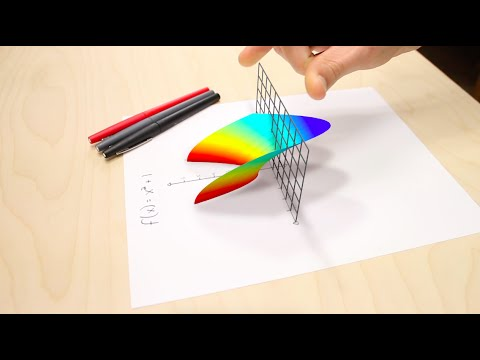
\includegraphics[height=6cm,width=1\textwidth,keepaspectratio]{im_video.jpg}}
        % \caption{Click on a picture for a video}
        \label{fig:im_video.jpg}
    \end{figure}
\end{frame}

\begin{frame}[t]{Complex numbers}
    \framesubtitle{Forms}
    \vspace{-0.5cm}
    \begin{columns}[T,onlytextwidth]
        \begin{column}{0.55\textwidth}
            \textbf{Rectangular form:} $z=x+iy,\ i^2=-1 $\\
            $Re(z)=x$ -- real part, $Im(z)=y$ -- imaginary part \\
            \textit{Example:} $z=5 + i6$ \\
            \textbf{Polar form:} $z=r\ cos(\phi) + i\ r\ sin(\phi) $, where \\
            $\phi = atan2(Im(z),Re(z))$; \\
            $r = |z|=\sqrt{x^2+y^2}$ -- magnitude \\
            \textit{Example:} $z=8\ cos(24)+i\ sin(24))$ \\
            \textbf{Exponential form:} $z=re^{i \phi}$ \\
            \textit{Example:} $z=6e^{i 2.5}$ \\
            \textbf{Euler formula:} \textit{transformation from exp. to polar} \\
            $e^{i\phi} = cos(\phi) + i\ sin(\phi)$
        \end{column}
        \begin{column}{0.44\textwidth}
            \vspace{-0.8cm}
            \begin{minipage}{0.58\textwidth}
                \centering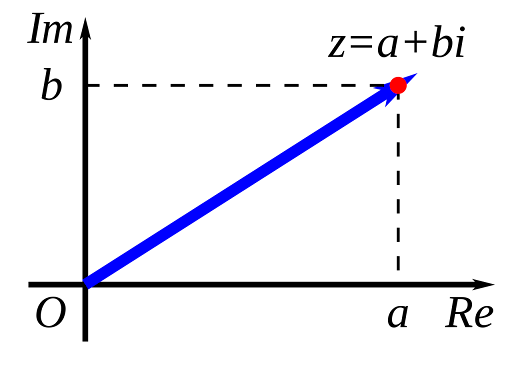
\includegraphics[width=\textwidth,keepaspectratio]{rectangular_form.png}
            \end{minipage}\hfill
            \begin{minipage}{0.40\textwidth}
                Rectangular form
                \label{fig:rectangular_form.png}
            \end{minipage}
            \vspace{-0.5cm}
            \begin{minipage}{0.58\textwidth}
                \centering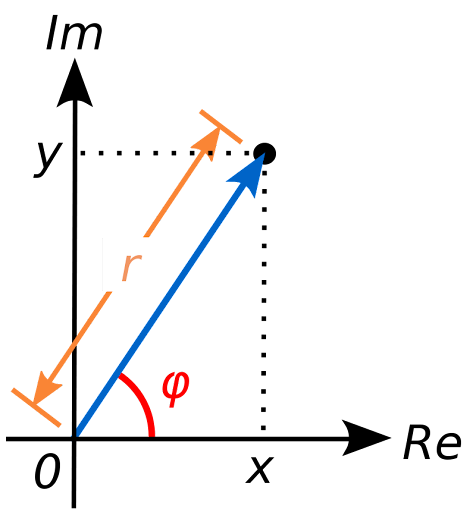
\includegraphics[height=4cm,width=\textwidth,keepaspectratio]{polar_form.png}
            \end{minipage}\hfill
            \begin{minipage}{0.40\textwidth}
                Polar or \\ Exponential form
                \label{fig:polar_form.png}
            \end{minipage}
        \end{column}
    \end{columns}
\end{frame}

\begin{frame}[t]{Complex numbers}
    \framesubtitle{Operations}
    \textbf{General Idea}: you should work with $Im$ and $Re$ part separately (you cannot sum or multiply them) \\
    \begin{itemize}
        \item \textit{Summarization and Subtraction} -- $(x_1 \pm iy_1) + (x_2 \pm iy_2) = (x_1 \pm x_2) + i(y_1\pm y_2)$
        \item \textit{Multiplication} -- $(x_1 + iy_1)(x_2 + iy_2) = (x_1x_2 - y_1y_2) + i(x_1y_2 + y_1x_2)$
        \item \textit{Division} -- $\dfrac{(x_2 + iy_2)}{(x_1 + iy_1)} = \dfrac{(x_1x_2 + y_1y_2)}{x_2^2 + y_2^2} + i\dfrac{(y_1x_2 - x_1y_2)}{x_2^2 + y_2^2} $
    \end{itemize}
\end{frame}

\begin{frame}[t]{Complex numbers}
    \framesubtitle{Complex conjugate}
    \vspace{-0.3cm}
    \begin{columns}[T,onlytextwidth]
        \begin{column}{0.7\textwidth}
            \textit{Complex conjugate} of complex number $z = x+ iy$ -- ${\bar  z}=x-iy$. Geometrically it's reflection of z about $Re$ axis.

            \textbf{Properties:}\\
            $Re(\bar{z}) = Re(z))$ and $|\bar{z}| = |z|$; \\
            $Im(\bar{z}) = -Im(z)$ and $arg\ \bar{z}\equiv -arg\ z (mod\ 2\pi)$ \\
            $z\bar{z} = x^2 + y^2 = |z|^2$ -- absolute square \\
            \textbf{Operations}
            \begin{itemize}
                \item  \textit{Summarization and Subtraction} -- ${\overline {z\pm w}}={\bar {z}}\pm {\bar {w}}$
                \item \textit{Multiplication} -- ${\overline {z\cdot w}}={\bar {z}}\cdot {\bar {w}}$
                \item \textit{Division} -- ${\overline {z/w}}={\bar {z}}/{\bar {w}}$
            \end{itemize}

        \end{column}
        \begin{column}{0.29\textwidth}
            \vspace{-0.5cm}
            \begin{figure}[H]
                \centering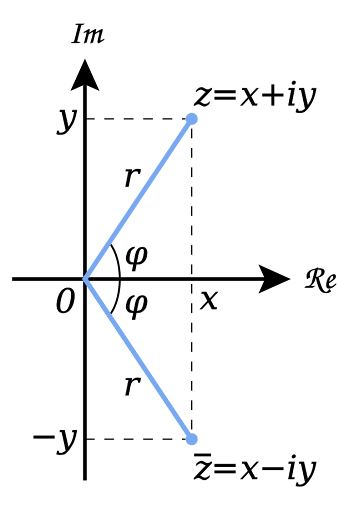
\includegraphics[height=5cm,width=1\textwidth,keepaspectratio]{conjugate.png}
                \caption*{Complex Conjugate}
                \label{fig:conjugate.png}
            \end{figure}
        \end{column}
    \end{columns}
\end{frame}

\begin{frame}[t]{Complex numbers}
\framesubtitle{Applications (1)}
\vspace{-0.4cm}
\large
\begin{block}{Typical reason}
    Most of the time for simplicity your calculations, except Quantum computing and some other topics.
\end{block}
    \begin{enumerate}
        \item \textit{Electromagnetism}: electric and magnetic fields as complex vector fields to describe electromagnetic waves. However, this is just a computational trick.
        \item \textit{Aerodynamics}: calculating wing shapes using Joukowsky transform.
        \item \textit{Geodesy}: Google Maps (from Geoid to 2d map).
        \item \textit{Quantum Computing}
    \end{enumerate}
\end{frame}

\begin{frame}[t]{Complex numbers}
    \framesubtitle{Applications (2): Video}
    \vspace{-0.6cm}
    \begin{figure}[H]
        \href{https://www.youtube.com/watch?v=JA_VZ8Frrvw}{
            \centering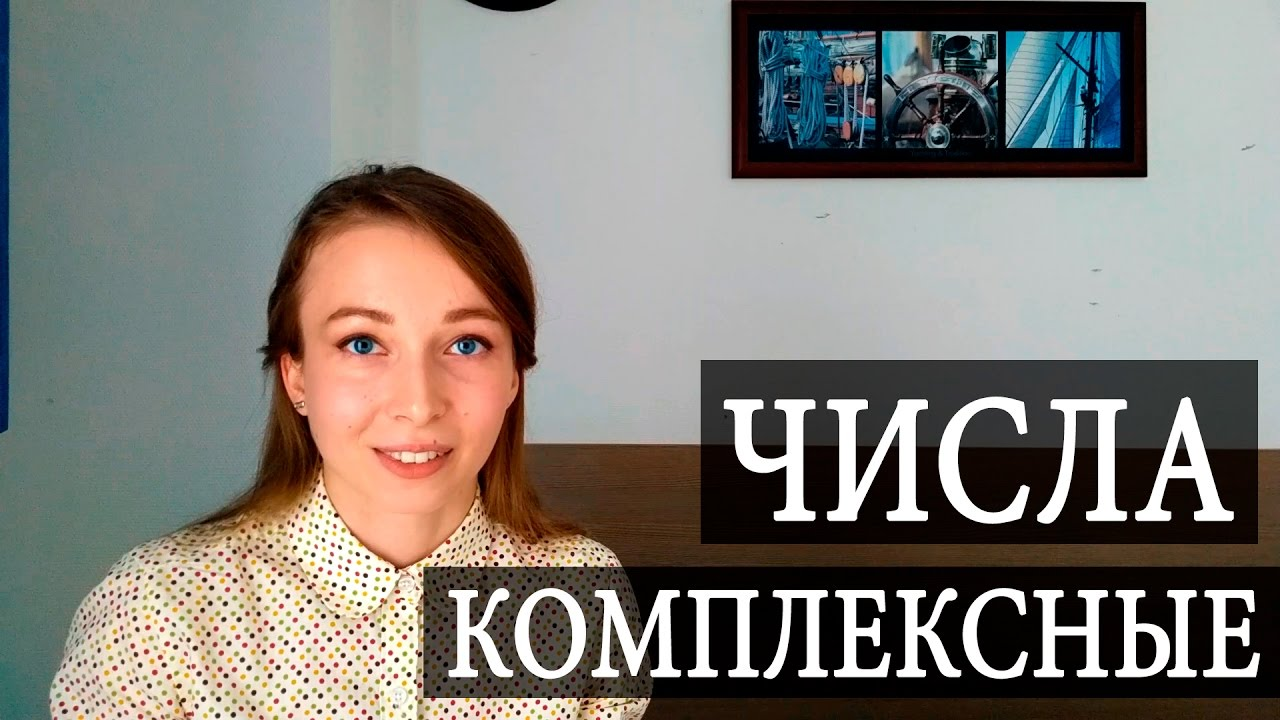
\includegraphics[height=6cm,width=1\textwidth,keepaspectratio]{com_video.jpg}}
        % \caption{Click on a picture for a video}
        \label{fig:com_video.jpg}
    \end{figure}
\end{frame}

\begin{frame}[t]{Complex numbers}
\framesubtitle{Applications(3): more about Quantum Computing (Links)}
\Large
\begin{itemize}
    \item \href{https://qiskit.org/textbook/ch-states/representing-qubit-states.html}{Representing Qubit States as complex numbers}
    \item \href{https://www.nature.com/articles/s41586-021-04160-4}{Why do we have to use complex numbers in Quantum computing (Nature paper)}
    \item \href{https://en.wikipedia.org/wiki/Bloch_sphere}{Bloch sphere is a geometrical representation of the pure state space of a two-level quantum mechanical system (qubit)}
\end{itemize}
\textit{If you are interested in the topic, you can ask \textbf{Stas Protasov}}.
    
\end{frame}

\begin{frame}[t]{Task 1}
    \framesubtitle{}
    \vspace{-0.6cm}
    \setbeamertemplate{itemize/enumerate body begin}{\large}
    \setbeamertemplate{itemize/enumerate subbody begin}{\large}
    \begin{multicols}{2}
        \begin{enumerate}
            \only<1,2>{ \item[1] For $z=\dfrac{1+i}{\sqrt{2}}$:\begin{itemize}
                    \item Compute $z^2$
                    \item Find $r$
                    \item Find $\phi$
                    \item Find $z$ in exponential form
                \end{itemize}}
                \only<1,3>{\item[2] \begin{itemize}
                    \item Find the 8 solutions to the equation $z^8 = 1$
                    \item Plot those 8 solutions in the complex plane
                \end{itemize}}
                \only<1,4>{\item[3] For $z = -1 + i\frac{1}{2}$ \begin{itemize}
                    \item Find complex conjugate ($\bar{z}$)
                    \item Find $z\bar{z}$
                    \item Find $z+\bar{z}$
                    \item Plot each result in the complex plane
                \end{itemize}}
                \only<1,5>{\item[4] Find: \begin{itemize}
                    \item $e^{i\frac{\pi}{2}}$
                    \item $e^{i\pi}$
                    \item $i^i$
                    \item Show each result in the complex plane
                \end{itemize}}
        \end{enumerate}
    \end{multicols}
    \only<2-5>{\alert{\Large Answer}\\}
    \only<2>{\begin{itemize}
        \item $z^2=i$
        \item $r=1$
        \item $\phi=45^\circ$
        \item $z=1e^{i \frac{\pi}{4}}$
    \end{itemize}}
    \only<3>{\href{https://www.kontrolnaya-rabota.ru/s/equal-one/any-uravnenie/expr/d2ceda2e3e26d3d04083ac82a3b37db3/}{Solution (rus)}:
    $\pm1;\ \pm i;\ \frac{\sqrt{2}}{2}\pm i \frac{\sqrt{2}}{2};\ -\frac{\sqrt{2}}{2}\pm i \frac{\sqrt{2}}{2};$}
    \only<4>{\begin{itemize}
        \item $\bar{z}=-1-i\frac{1}{2}$
        \item $z\bar{z}=1.25$
        \item $z+\bar{z}=-2$
    \end{itemize}}
    \only<5>{\begin{itemize}
        \item $e^{i\frac{\pi}{2}}=i$
        \item $e^{i\pi}=-1$
        \item $i^i=e^{ln(i^i)}=e^{i\ ln(i)};\ \left\{\begin{matrix*}[l]
            i=e^{i\frac{\pi}{2}} \text{-- \small \textit{from 1-st bullet}}\\ln(i)=ln(e^{i\frac{\pi}{2})}
        \end{matrix*}\right. \rightarrow i\frac{\pi}{2}=ln(i);\ e^{i\ ln(i)}=e^{-\frac{\pi}{2}}=0.208$ 
    \end{itemize}}

    \setbeamertemplate{itemize/enumerate body begin}{\normalsize}
    \setbeamertemplate{itemize/enumerate subbody begin}{\normalsize}
\end{frame}

\begin{frame}[t]{Complex Matrices}
\framesubtitle{Common and Special}
\vspace{-0.3cm}
    \large \textit{Many concepts have a new name, but old meaning}:
    \vspace{-0.25cm}
    \begin{itemize}
        \item $A^T \rightarrow A^H$; $A^H = \bar{A}^T$, $H$ -- conjugate $T$; \textit{Exp:} {\scriptsize $\begin{bmatrix}
        1 & -2-i & 5 \\
        1+i & i & 4-2i 
        \end{bmatrix} \rightarrow \begin{bmatrix}
        1 & 1-i \\
        -2+i & -i \\ 
        5 & 4+2i 
        \end{bmatrix}$}
        \vspace{-0.3cm}
        \item $Q \rightarrow U$; $U=Q$, where $U$ -- Unitary matrix
    \end{itemize}
    \vspace{-0.38cm}
    \begin{figure}[H]
        \centering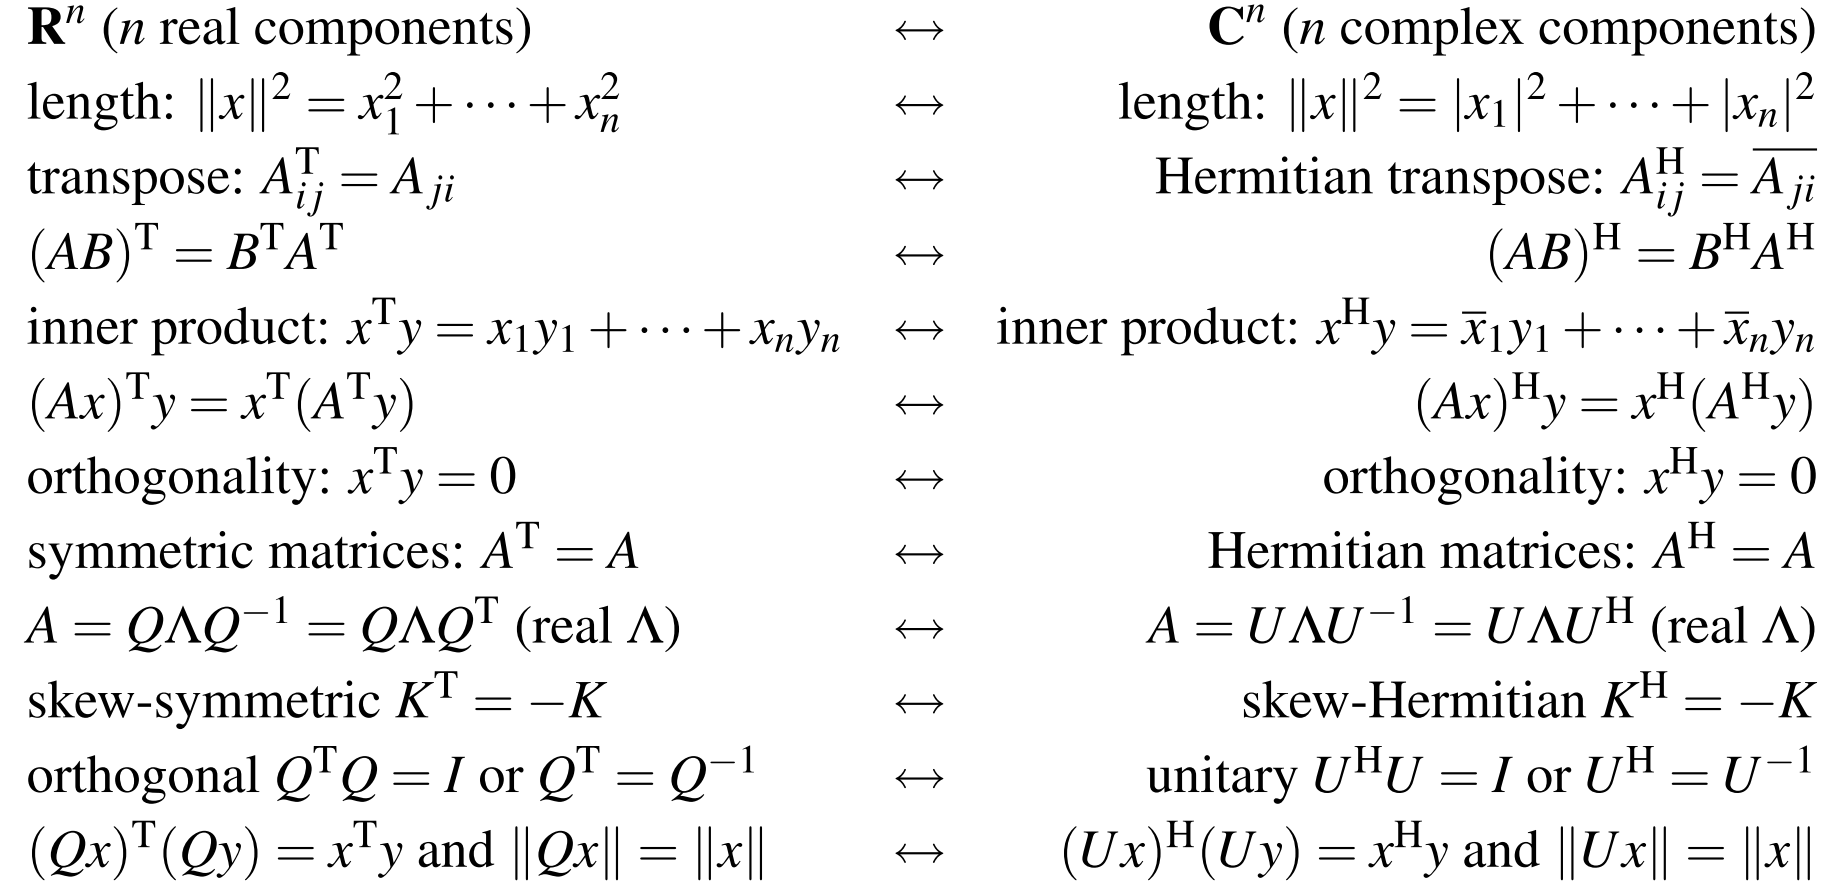
\includegraphics[height=4.2cm,width=1\textwidth,keepaspectratio]{complex_matrices.png}
        % \caption{caption_name}
        \label{fig:complex_matrices.png}
    \end{figure}
\end{frame}

\begin{frame}[t]{Task 2}
    \framesubtitle{}
    \begin{figure}[H]
        \centering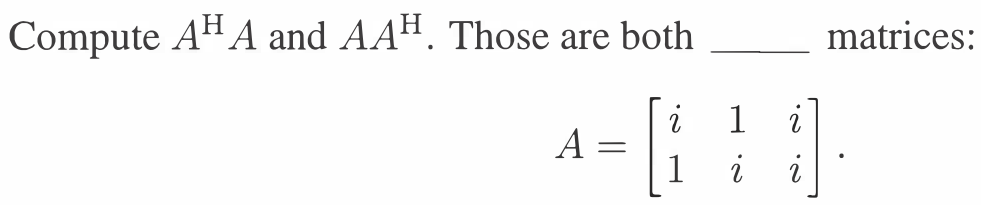
\includegraphics[height=3cm,width=1\textwidth,keepaspectratio]{2.png}
        % \caption{caption_name}
        \label{fig:2.png}
    \end{figure}
    \uncover<2->{
        \vspace{-0.3cm}
        \alert{\Large Answer}
        \begin{figure}[H]
            \centering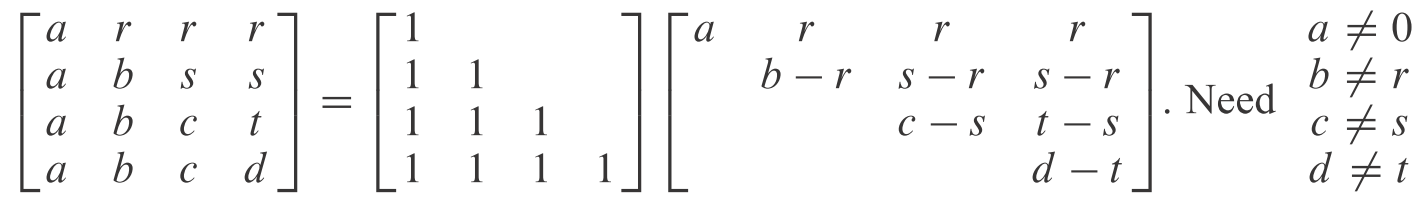
\includegraphics[height=3cm,width=1\textwidth,keepaspectratio]{2ans.png}
            % \caption{caption_name}
            \label{fig:2ans.png}
        \end{figure}
    }
\end{frame}

\begin{frame}[t]{Task 3}
    \framesubtitle{}
    \begin{figure}[H]
        \centering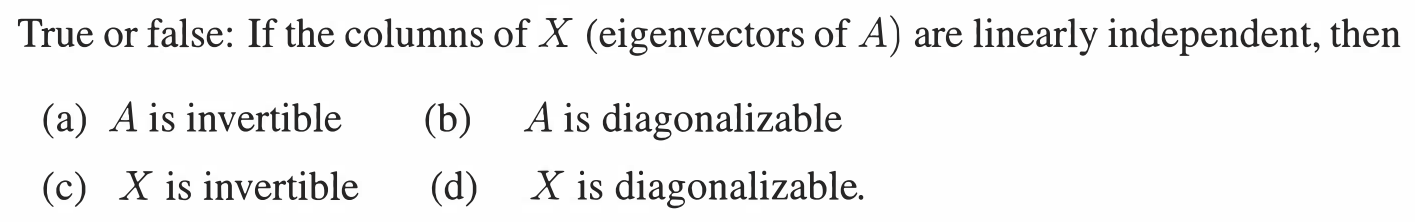
\includegraphics[height=3cm,width=1\textwidth,keepaspectratio]{3.png}
        % \caption{caption_name}
        \label{fig:3.png}
    \end{figure}
    \uncover<2->{
        \alert{\Large Answer}
        \begin{figure}[H]
            \centering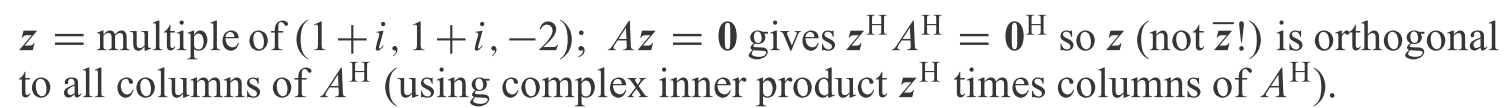
\includegraphics[height=3cm,width=1\textwidth,keepaspectratio]{3ans.png}
            % \caption{caption_name}
            \label{fig:3ans.png}
        \end{figure}
    }
\end{frame}

\begin{frame}[t]{Task 4}
    \framesubtitle{}
    \begin{figure}[H]
        \centering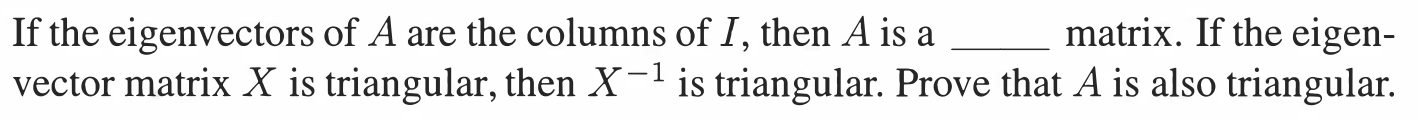
\includegraphics[height=3cm,width=1\textwidth,keepaspectratio]{4.png}
        % \caption{caption_name}
        \label{fig:4.png}
    \end{figure}
    \uncover<2->{
        \alert{\Large Answer}
        \begin{figure}[H]
            \centering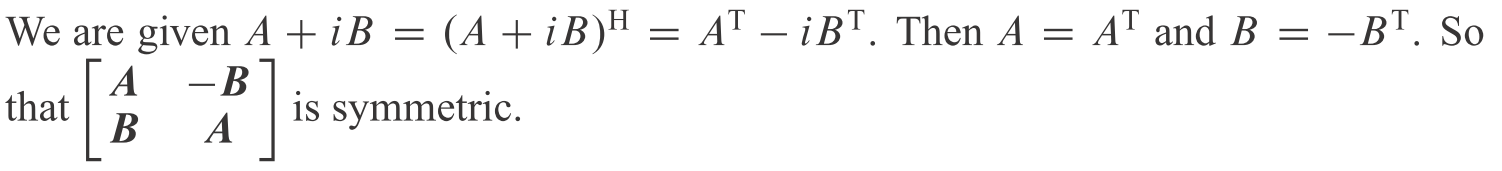
\includegraphics[height=3cm,width=1\textwidth,keepaspectratio]{4ans.png}
            % \caption{caption_name}
            \label{fig:4ans.png}
        \end{figure}
    }
\end{frame}

\begin{frame}[t]{Reference material}
    \framesubtitle{}
    \Large
    \begin{itemize}
        \item \href{https://www.youtube.com/watch?v=M0Sa8fLOajA&list=PL49CF3715CB9EF31D&index=27}{Lecture 26}
        \item \href{https://youtu.be/Jkv-55ndVYY}{Complex Numbers Part Imaginary, but Really Simple}
        \item \textit{"Linear Algebra and Applications", pdf pages 322--335 }\\ Complex numbers and matrices
        \item \textit{"Introduction to Linear Algebra", pdf pages 504--519 }\\ Complex numbers and matrices
        \item \href{https://programforyou.ru/calculators/complex-calculator}{Complex Numbers calculator}
    \end{itemize}
\end{frame}

\fbckg{fibeamer/figs/last_page.png}
\frame[plain]{}

\end{document}